%%%%%%%%%%%%%%%%%%%%%%%%%%%%%%%%%%%%%%%%%%%%%%%%%%%%%%%%%%%%%%%%%%%%%
%%                                                                 %%
%% Please do not use \input{...} to include other tex files.       %%
%% Submit your LaTeX manuscript as one .tex document.              %%
%%                                                                 %%
%% All additional figures and files should be attached             %%
%% separately and not embedded in the \TeX\ document itself.       %%
%%                                                                 %%
%%%%%%%%%%%%%%%%%%%%%%%%%%%%%%%%%%%%%%%%%%%%%%%%%%%%%%%%%%%%%%%%%%%%%

%%\documentclass[referee,sn-basic]{sn-jnl}% referee option is meant for double line spacing

%%=======================================================%%
%% to print line numbers in the margin use lineno option %%
%%=======================================================%%

%%\documentclass[lineno,sn-basic]{sn-jnl}% Basic Springer Nature Reference Style/Chemistry Reference Style

%%======================================================%%
%% to compile with pdflatex/xelatex use pdflatex option %%
%%======================================================%%

%%\documentclass[pdflatex,sn-basic]{sn-jnl}% Basic Springer Nature Reference Style/Chemistry Reference Style

%%\documentclass[sn-basic]{sn-jnl}% Basic Springer Nature Reference Style/Chemistry Reference Style
\documentclass[sn-mathphys]{sn-jnl}% Math and Physical Sciences Reference Style
%%\documentclass[sn-aps]{sn-jnl}% American Physical Society (APS) Reference Style
%%\documentclass[sn-vancouver]{sn-jnl}% Vancouver Reference Style
%%\documentclass[sn-apa]{sn-jnl}% APA Reference Style
%%\documentclass[sn-chicago]{sn-jnl}% Chicago-based Humanities Reference Style
%%\documentclass[sn-standardnature]{sn-jnl}% Standard Nature Portfolio Reference Style
%%\documentclass[default]{sn-jnl}% Default
%%\documentclass[default,iicol]{sn-jnl}% Default with double column layout

%%%% Standard Packages
%%<additional latex packages if required can be included here>
%%%%

%%%%%=============================================================================%%%%
%%%%  Remarks: This template is provided to aid authors with the preparation
%%%%  of original research articles intended for submission to journals published
%%%%  by Springer Nature. The guidance has been prepared in partnership with
%%%%  production teams to conform to Springer Nature technical requirements.
%%%%  Editorial and presentation requirements differ among journal portfolios and
%%%%  research disciplines. You may find sections in this template are irrelevant
%%%%  to your work and are empowered to omit any such section if allowed by the
%%%%  journal you intend to submit to. The submission guidelines and policies
%%%%  of the journal take precedence. A detailed User Manual is available in the
%%%%  template package for technical guidance.
%%%%%=============================================================================%%%%

\jyear{2025}%

%% as per the requirement new theorem styles can be included as shown below
\theoremstyle{thmstyleone}%
\newtheorem{theorem}{Theorem}%  meant for continuous numbers
%%\newtheorem{theorem}{Theorem}[section]% meant for sectionwise numbers
%% optional argument [theorem] produces theorem numbering sequence instead of independent numbers for Proposition
\newtheorem{proposition}[theorem]{Proposition}%
%%\newtheorem{proposition}{Proposition}% to get separate numbers for theorem and proposition etc.

\theoremstyle{thmstyletwo}%
\newtheorem{example}{Example}%
\newtheorem{remark}{Remark}%

\theoremstyle{thmstylethree}%
\newtheorem{definition}{Definition}%

\raggedbottom
%%\unnumbered% uncomment this for unnumbered level heads
\usepackage{algorithm}
\usepackage{algpseudocode}
\usepackage{amsmath}
\usepackage{colortbl}
\usepackage{color}
\usepackage{makecell}
\usepackage{multirow}
\renewcommand{\algorithmicrequire}{\textbf{Input:}}  % Use Input in the format of Algorithm
\renewcommand{\algorithmicensure}{\textbf{Output:}} % Use Output in the format of Algorithm
%% The amssymb package provides various useful mathematical symbols
\usepackage{amssymb}
\usepackage{subfigure}
\begin{document}

\title{Segmentation-Enhanced Diffusion: Achieving High-Fidelity Thangka Generation through Iconometric Rule Encoding}

%%=============================================================%%
%% Prefix	-> \pfx{Dr}
%% GivenName	-> \fnm{Joergen W.}
%% Particle	-> \spfx{van der} -> surname prefix
%% FamilyName	-> \sur{Ploeg}
%% Suffix	-> \sfx{IV}
%% NatureName	-> \tanm{Poet Laureate} -> Title after name
%% Degrees	-> \dgr{MSc, PhD}
%% \author*[1,2]{\pfx{Dr} \fnm{Joergen W.} \spfx{van der} \sur{Ploeg} \sfx{IV} \tanm{Poet Laureate}
%%                 \dgr{MSc, PhD}}\email{iauthor@gmail.com}
%%=============================================================%%

\author[1,2,3]{\fnm{Fubo} \sur{WANG}}\email{1814602213@qq.com}

\author*[1,2,3]{\fnm{Shengling} \sur{GENG}}\email{geng$\_$sl@126.com}
\equalcont{These authors contributed equally to this work.}

\affil*[1]{\orgdiv{School of Computer Science}, \orgname{Qinghai Normal University}, \orgaddress{\street{Hutai}, \city{Xining}, \postcode{810008}, \state{Qinghai}, \country{China}}}

\affil[2]{\orgdiv{Academy of Plateau Science and Sustainability}, \orgname{People's Government Of Qinghai Province ${\rm{\& }}$ Beijing Normal University}, \orgaddress{\street{Haihu}, \city{Xining}, \postcode{810004}, \state{Qinghai}, \country{China}}}

\affil[3]{\orgdiv{The State Key Laboratory of Tibetan Intelligent Information Processing and Application}, \orgname{Qinghai Normal University}, \orgaddress{\street{Hutai}, \city{Xining}, \postcode{810008}, \state{Qinghai}, \country{China}}}

%%==================================%%
%% sample for unstructured abstract %%
%%==================================%%

\abstract{Thangka painting, a precious heritage of Tibetan Buddhist art, adheres strictly to complex iconometric rules outlined in sacred canons. Traditional manual creation methods face challenges in efficiency and cultural inheritance. This paper introduces TKSegDiff, a semantic segmentation-guided diffusion model designed for high-fidelity Thangka generation. By encoding traditional iconometric rules into dynamic embeddings and integrating them via cross-attention mechanisms, TKSegDiff ensures generated images comply with religious conventions. A ResNet152-based segmentation network, enhanced with a TKS2EA module, achieves precise element segmentation. Experiments on the TK-10K dataset demonstrate that TKSegDiff reduces the FID score by 29.58\% compared to Stable Diffusion and 23.80\% compared to BAGEL, with 75\% of generated results certified by Thangka artists. This research provides an effective solution for digital preservation of Thangka art and offers a structured generation framework applicable to other artistic image synthesis tasks. Code: https://github.com/HeHuangAI/TKSegDiff.}

%%================================%%
%% Sample for structured abstract %%
%%================================%%
\keywords{Thangka Generation, Diffusion Models, Semantic Segmentation, Structured Generation, Cultural Heritage Preservation}

%%\pacs[JEL Classification]{D8, H51}

%%\pacs[MSC Classification]{35A01, 65L10, 65L12, 65L20, 65L70}

\maketitle

\section{Introduction}
As a gem of Tibetan Buddhist art, Thangka \cite{b1} painting strictly adheres to religious canons such as 'The Sacred Canon of Measurements for Thangka Buddha Figures' \cite{b2}, which imposes rigorous specifications on Buddha proportions, ritual object placement, and color symbolism. The traditional painting process is illustrated in Fig.~\ref{fig1}. In recent years, the demand for digital preservation \cite{b3,b4,b5} has surged, yet traditional Thangka creation relies on decades of artisan expertise, resulting in inefficiency and a risk of cultural discontinuity. Although Generative Adversarial Networks (GANs) \cite{b6} and diffusion models \cite{b7} have advanced artistic image generation \cite{b8,b9}, existing methods still face challenges in synthesizing Thangka-a highly structured and semantically dense cultural heritage. Lack of Cultural Rules: Mainstream generative models rely on text prompts and fail to encode complex spatial constraints from the Iconometric Sutra, such as "symmetrical Buddha proportions," leading to distorted figures and misplaced ritual objects (Fig.~\ref{fig2}(b)). Fine-Grained Semantic Loss: Thangka’s decorative elements require pixel-level precision, but generic segmentation-guided methods \cite{b10,b11} underperform on dense small objects, causing semantic confusion. Global Incoherence: Existing methods lack explicit modeling of Thangka’s hierarchical structure ("deity-background-ornament" relationships), resulting in locally realistic but globally inconsistent outputs.

To address these issues, we propose TKSegDiff, a semantic segmentation-guided diffusion model for high-quality Thangka image generation. First, TKSegDiff encodes iconometric rules into dynamic embedding vectors and injects them into the diffusion model via cross-attention mechanisms, enforcing religious compliance during denoising. Second, we integrate a task-driven TKS2EA module into a ResNet 152 \cite{b12} backbone, leveraging multi-scale feature aggregation and spatial-semantic dual attention to achieve 85.36\% mIoU in segmenting Thangka-specific elements. Finally, a feature fusion module dynamically adjusts the generation process to ensure global cultural consistency.

Experiments on our TK-10K dataset (10,000 pixel-level annotated Thangka images) show that our method reduces the FID score decreased by 29.58\% compared to Stable Diffusion and 23.80\% compared to BAGEL. In blind tests by Tibetan cultural experts, 75\% of generated results were deemed "religiously compliant." Our work not only provides a novel solution for intangible cultural heritage digitization but also introduces a structured prior injection mechanism applicable to other religious art generation tasks, such as Dunhuang murals and Christian iconography.

\begin{figure}[htbp]
	\centerline{\includegraphics[width=0.9\linewidth]{fig1.png}}
	\caption{The drawing process of Thangka.}
	\label{fig1}
\end{figure}
\begin{figure}[htbp]
	\centerline{\includegraphics[width=1\linewidth]{fig2.png}}
	\caption{Thangka image generation comparison: (a): Real pre-training samples; (b, c): Results from baseline methods; (d): Our method’s output. Our approach achieves superior detail preservation and artistic fidelity.}
	\label{fig2}
\end{figure}
The key \textbf{contributions} of this work are summarized as follows:
\begin{itemize}
	\item For the first time, the traditional iconometric rules of Thangka are transformed into learnable conditional embeddings (tokens) and incorporated into the U-Net of the diffusion model through a cross-attention mechanism. This approach ensures that the generated Thangka images comply with religious rituals and artistic standards, effectively addressing structural distortions and proportional inaccuracies that may occur in existing generation methods;
	\item A semantic segmentation network for Thangka images is proposed, which is based on ResNet 152 and incorporates the TKS2EA module. This network accurately extracts local semantic information from Thangka images. The TKS2EA module enhances feature extraction through attention mechanisms, improving segmentation accuracy and providing pixel-level semantic guidance for subsequent generation;
	\item During the reverse denoising process of the diffusion model, semantic labels provided by the TKSS(Thangka Semantic Segmentation) module are utilized to refine the generation of different regions separately. This approach significantly improves the structural accuracy and detail quality of the generated images;
	\item A feature fusion module is introduced at the final stage of the generation pipeline to integrate local semantic information with global style features. This ensures that the generated Thangka images maintain overall harmony, natural coloring, and conformity with traditional aesthetic standards.
\end{itemize}	
%\captionsetup[figure]{singlelinecheck=off}

\section{Related Work}
\subsection{Artificial Intelligence Generated Content}
\textbf{GANs. }With recent advances in deep learning, GANs have been applied to Thangka style transfer, yet the generated results often violate religious canons. StyleGAN\cite{b13}, a milestone series of models developed by NVIDIA in 2020, is renowned for its high-quality and controllable image generation. However, due to the lack of explicit structural constraints in its latent space, it struggles to learn long-tail features characteristic of Thangka art. SPADE (Spatially-Adaptive Denormalization) \cite{b14}, proposed in 2019, is a conditional normalization-based GAN that precisely controls local details through spatially-adaptive normalization of semantic segmentation maps. However, the religious artistry of Thangka requires extremely fine textures and geometric symmetry, which SPADE's normalization mechanism fails to fully capture, resulting in blurred or structurally distorted outputs. Wang et al.\cite{b15} proposed a GAN-based method for coloring Thangka line drawings in 2023, but the style diversity is limited due to the line-drawing guidance. Komeda et al.\cite{b16} developed an automated generation method based on parameterized motifs and layout subdivision for designing complex Acanthus ornamentation patterns (commonly found in classical architecture). The system allows style and layout control through user-defined parameters, facilitating artistic creation and digital cultural heritage preservation, though it performs particularly well with symmetrical patterns.

\textbf{Transformer. }Lin et al.\cite{b17} introduced an Efficient Attention Pyramid Transformer (EAPT) featuring a hierarchical pyramid structure to optimize computational efficiency. By integrating local and global attention mechanisms for multi-scale image feature processing, this architecture demonstrates effectiveness in image classification and super-resolution tasks while maintaining performance with reduced computational resources. Zhang et al.\cite{b18} presented a Mutual Attention-based Transformer architecture for image anomaly detection. By capturing interactions between local and global image features, the method enhances sensitivity to abnormal regions and improves detection accuracy, making it suitable for industrial quality inspection and medical image analysis scenarios.

\textbf{Diffusion Models.} Diffusion models have become the mainstream approach for image generation, achieving high-quality synthesis through iterative denoising. In artistic generation, models like Stable Diffusion \cite{b19} and DALL·E \cite{b20} have demonstrated strong capabilities but still face practical challenges. Karlo \cite{b21}, introduced by Kakao Brain in 2024, is a text-to-image generation model based on diffusion architecture, similar to DALL·E 3. It achieves high-quality generation through large-scale multimodal training (text-image pairs) and optimizes generation speed and detail preservation. However, Karlo's latent space control struggles to enforce pixel-level compositional constraints, disrupting the symmetry and proportions of Buddha figures.

FLUX.1 \cite{b22}, released by Stability AI in 2024, is an upgraded version of the Stable Diffusion series. While it significantly improves text comprehension, image quality, and controllable generation, FLUX.1 still encounters issues such as element overlap, disproportions, and perspective errors in complex layouts, requiring extensive ControlNet constraints for partial mitigation.

BAGEL (Bootstrapped Attention-Guided Generative Latent Diffusion) \cite{b23}, proposed by ByteDance's Seed team in 2024, is a novel text-to-image model based on an improved Latent Diffusion Model (LDM) architecture. It incorporates bootstrapped attention mechanisms and dynamic latent space optimization. Although BAGEL excels in general text-to-image generation, particularly in complex semantic binding, Thangka's religious norms, material specificity, and compositional complexity impose higher demands.

Stable Diffusion 3 \cite{b24}, the latest diffusion model by Stability AI, significantly improves image quality, text understanding, and controllability over its predecessor (SDXL). However, it exhibits noticeable structural instability in complex compositions, often misplacing elements in Thangka generation. These general diffusion models rely on text prompts and fail to encode the strict structural constraints of religious art (Thangka's iconometric rules), leading to disproportioned Buddha figures or misplaced ritual objects. While methods like ControlNet \cite{b25} and T2I-Adapter \cite{b26} attempt to introduce spatial conditioning, they remain inadequate for fine-grained generation of Thangka's dense decorations. Moreover, most existing models are trained on Western art data, causing deviations in color and composition from traditional Thangka styles. In contrast, our work introduces an iconometric token injection mechanism, embedding religious canons as learnable priors into the diffusion model to ensure cultural compliance.

\subsection{Person Image Generation}
Zhang et al.\cite{b27} proposed a method for generating frontal portrait images from arbitrary human body viewpoints. This approach combines GANs to address occlusion and deformation challenges during viewpoint transformation, with potential applications in virtual try-on and identity recognition systems. Jiang et al.\cite{b28} created the PhotoHelper system that provides portrait photography guidance through deep feature retrieval and fusion technology. The system analyzes input images, retrieves similar examples from databases, and generates optimization suggestions by fusing aesthetic features to assist non-professional users in capturing high-quality portraits.

\subsection{Semantic Segmentation-Guided Generation}
Semantic segmentation is commonly used in generative tasks for structural control. SPADE \cite{b14} integrates semantic maps into the generation network via conditional normalization layers but relies on fixed segmentation labels, making it unsuitable for Thangka's complex small-object distributions. Semantic Diffusion Guidance \cite{b29} introduces segmentation-based gradient guidance during diffusion, enhancing semantic-text alignment through cross-attention. ControlNet \cite{b25} fine-tunes the diffusion model's encoder to support low-dimensional inputs. MaskDiffusion \cite{b30} combines diffusion models with dynamic mask optimization but performs poorly in global coordination of multi-scale objects.

Our method jointly optimizes diffusion models and semantic segmentation while incorporating iconometric priors. The proposed TKSS module is specifically designed for Thangka's semantic characteristics, significantly improving segmentation accuracy (mIoU +60\%) and enhancing generation quality through closed-loop feedback. It surpasses existing works in both cultural compliance and artistic quality.

\section{METHODOLOGY}
\subsection{Overview}
Fig.~\ref{fig3} illustrates the overall framework of our proposed semantic segmentation-guided Thangka image diffusion method, TKSegDiff. Designed to address the inherent complexity of Thangka imagery and its strict religious iconographic conventions, our approach employs a three-stage optimization strategy: First, traditional iconometric rules are encoded as dynamic embedding vectors and injected into the diffusion model via cross-attention mechanisms, ensuring generated content adheres to religious standards. Second, we construct a semantic segmentation network based on ResNet 152 and a TKS2EA module, which achieves precise segmentation of key elements through multi-scale feature aggregation and dual spatial-semantic attention mechanisms. Finally, a feature fusion module dynamically regulates the diffusion process to harmonize local details with overall compositional style. The following sections elaborate on each module.
\begin{figure}[htbp]
	\centerline{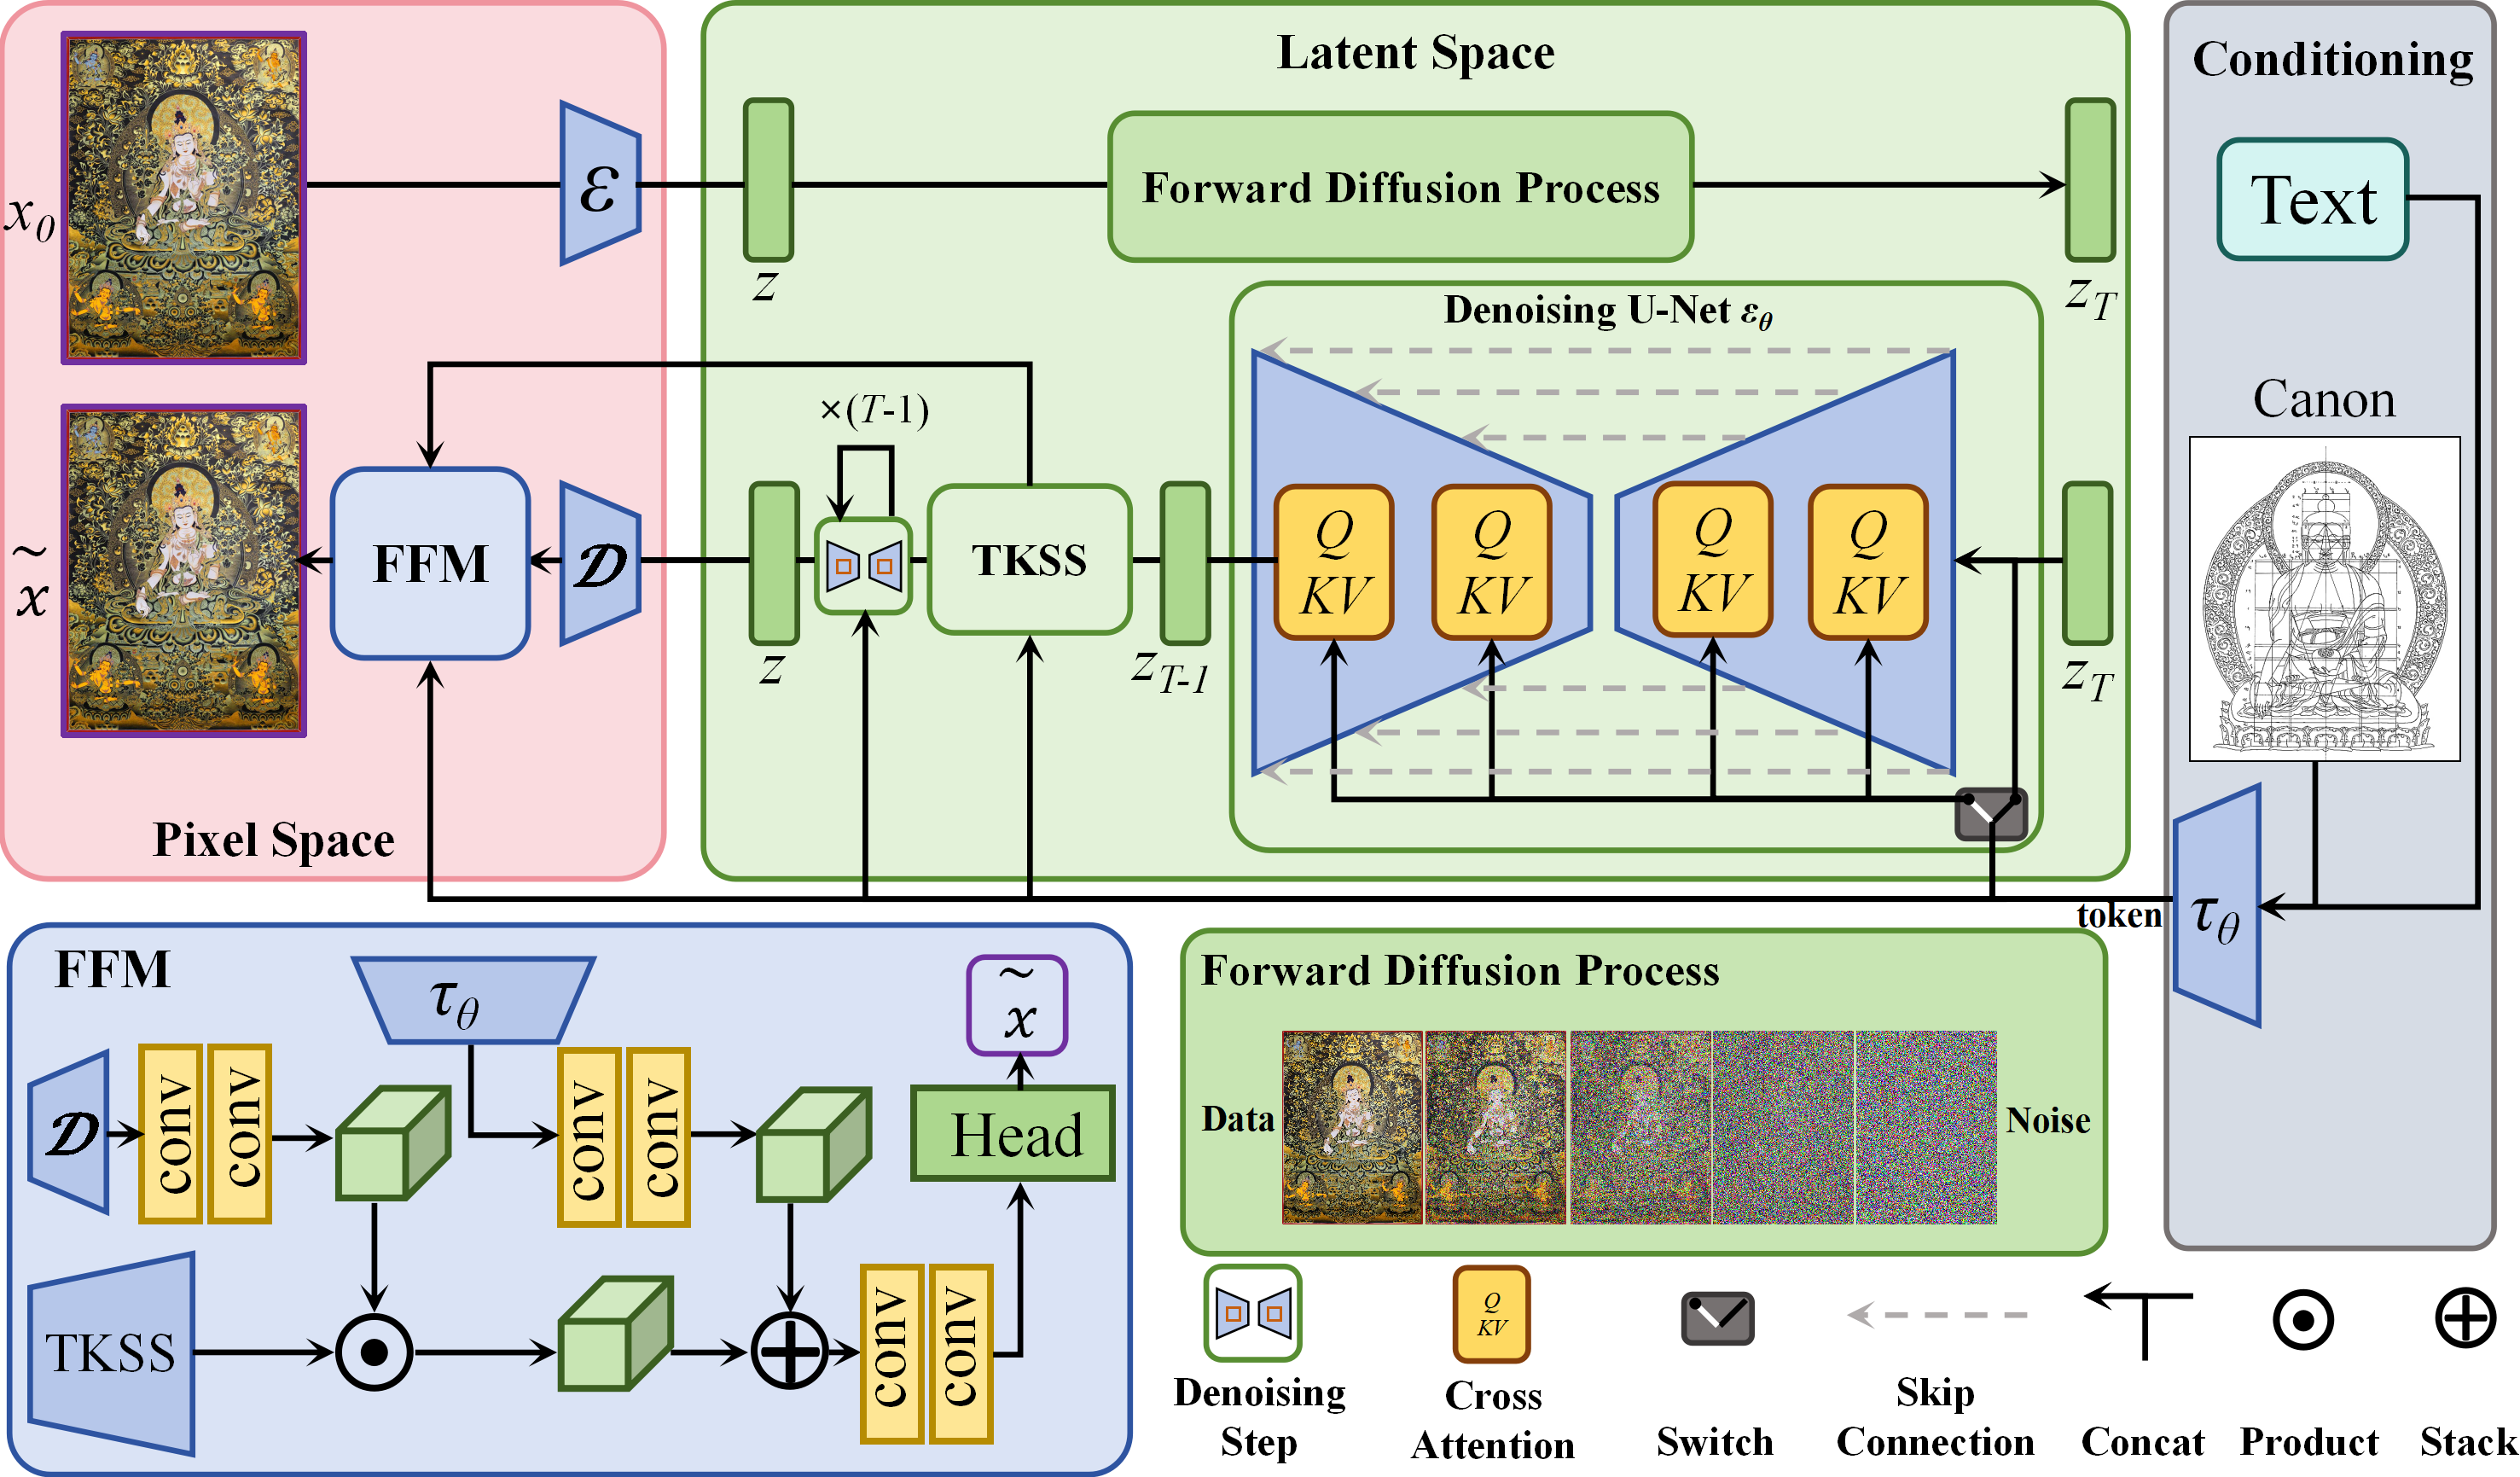
\includegraphics[width=1\linewidth]{fig3.png}}
	\caption{Overall framework.}
	\label{fig3}
\end{figure}
\subsection{Forward Diffusion Process}
The forward diffusion process follows the standard Denoising Diffusion Probabilistic Model (DDPM) \cite{b31} framework, gradually corrupting the original Thangka image $ x_0 $ into Gaussian noise $ x_T $ through a Markov chain of T diffusion steps.
\begin{equation}
	q({\bf{x}}t \vert {\bf{x}}t - 1) = N({\bf{x}}t;\sqrt {1 - {\beta _t}({\bf{m}})} {\bf{x}}t - 1,{\beta _t}({\bf{m}}){\bf{I}})
	\label{eq1}
\end{equation}
To better adapt to the unique characteristics of Thangka images, we propose a culturally-aware noise scheduling strategy. Recognizing that key regions in Thangka (such as Buddha faces, attire, and ritual objects) require higher preservation of structural details while backgrounds can tolerate stronger noise, we design a spatially-adaptive noise schedule $ {\beta _t}(m) $:
\begin{equation}
	{\beta _t}({\bf{m}}) = {\beta _{{\rm{base}}}} \cdot \left( {1 + \alpha  \cdot m} \right)
	\label{eq2}
\end{equation}
where $ m $ represents the iconometric mask ($ m=0.8 $ for Buddha regions, $ m=0.2 $ for background); $ \alpha $ is a learnable parameter controlling the degree of cultural adaptation; $ {\beta _t} $ is the standard noise schedule.

At each timestep $ t $, the noisy image $ {x_t} $ is generated through:
\begin{equation}
	{{\bf{x}}_t} = \sqrt {{{\bar \alpha }_t}} {{\bf{x}}_0} + \sqrt {1 - {{\bar \alpha }_t}} \varepsilon ,\;\;\;{\kern 1pt} \varepsilon  \in (0,{\bf{I}}) 
	\label{eq3}
\end{equation}
where $\bar{\alpha}_t=\prod_{s=1}^t(1-\beta_s(\mathbf{m}))$
\subsection{Reverse Denoising Process}
The reverse denoising process employs a U-Net to predict noise $ {\varepsilon _\theta } $, guided by both iconometric constraint injection and semantic segmentation. First, we transform the iconometric constraints from 'The Sacred Canon of Measurements for Thangka Buddha Figures' into learnable tokens. Specifically, the canonical rules are encoded as a token set $\mathbf{T}_m\in\mathbb{R}^{K\times d}$, where $ K=20 $ represents the number of rules and $ d=768 $ denotes the embedding dimension.

These constraints are injected into the U-Net through its cross-attention layers, formulated as:
\begin{equation}
	{\rm{Attention}}(Q,K,V) = {\rm{Softmax}}\left( {\frac{{Q{{[K;{{\bf{T}}_m}]}^T}}}{{\sqrt d }}} \right)[V;{{\bf{T}}_m}]
	\label{eq4}
\end{equation}
where $ Q $, $ K $, and $ V $ are the query, key, and value matrices of U-Net.
\subsection{TKSS Module}
\subsubsection{Backbone Network}
The TKSS network innovatively integrates attention mechanisms, local fine-detail modeling, global context awareness, and semantic edge context into a unified framework. As shown in Fig.~\ref{fig4}. 
\begin{figure}[htbp]
	\centerline{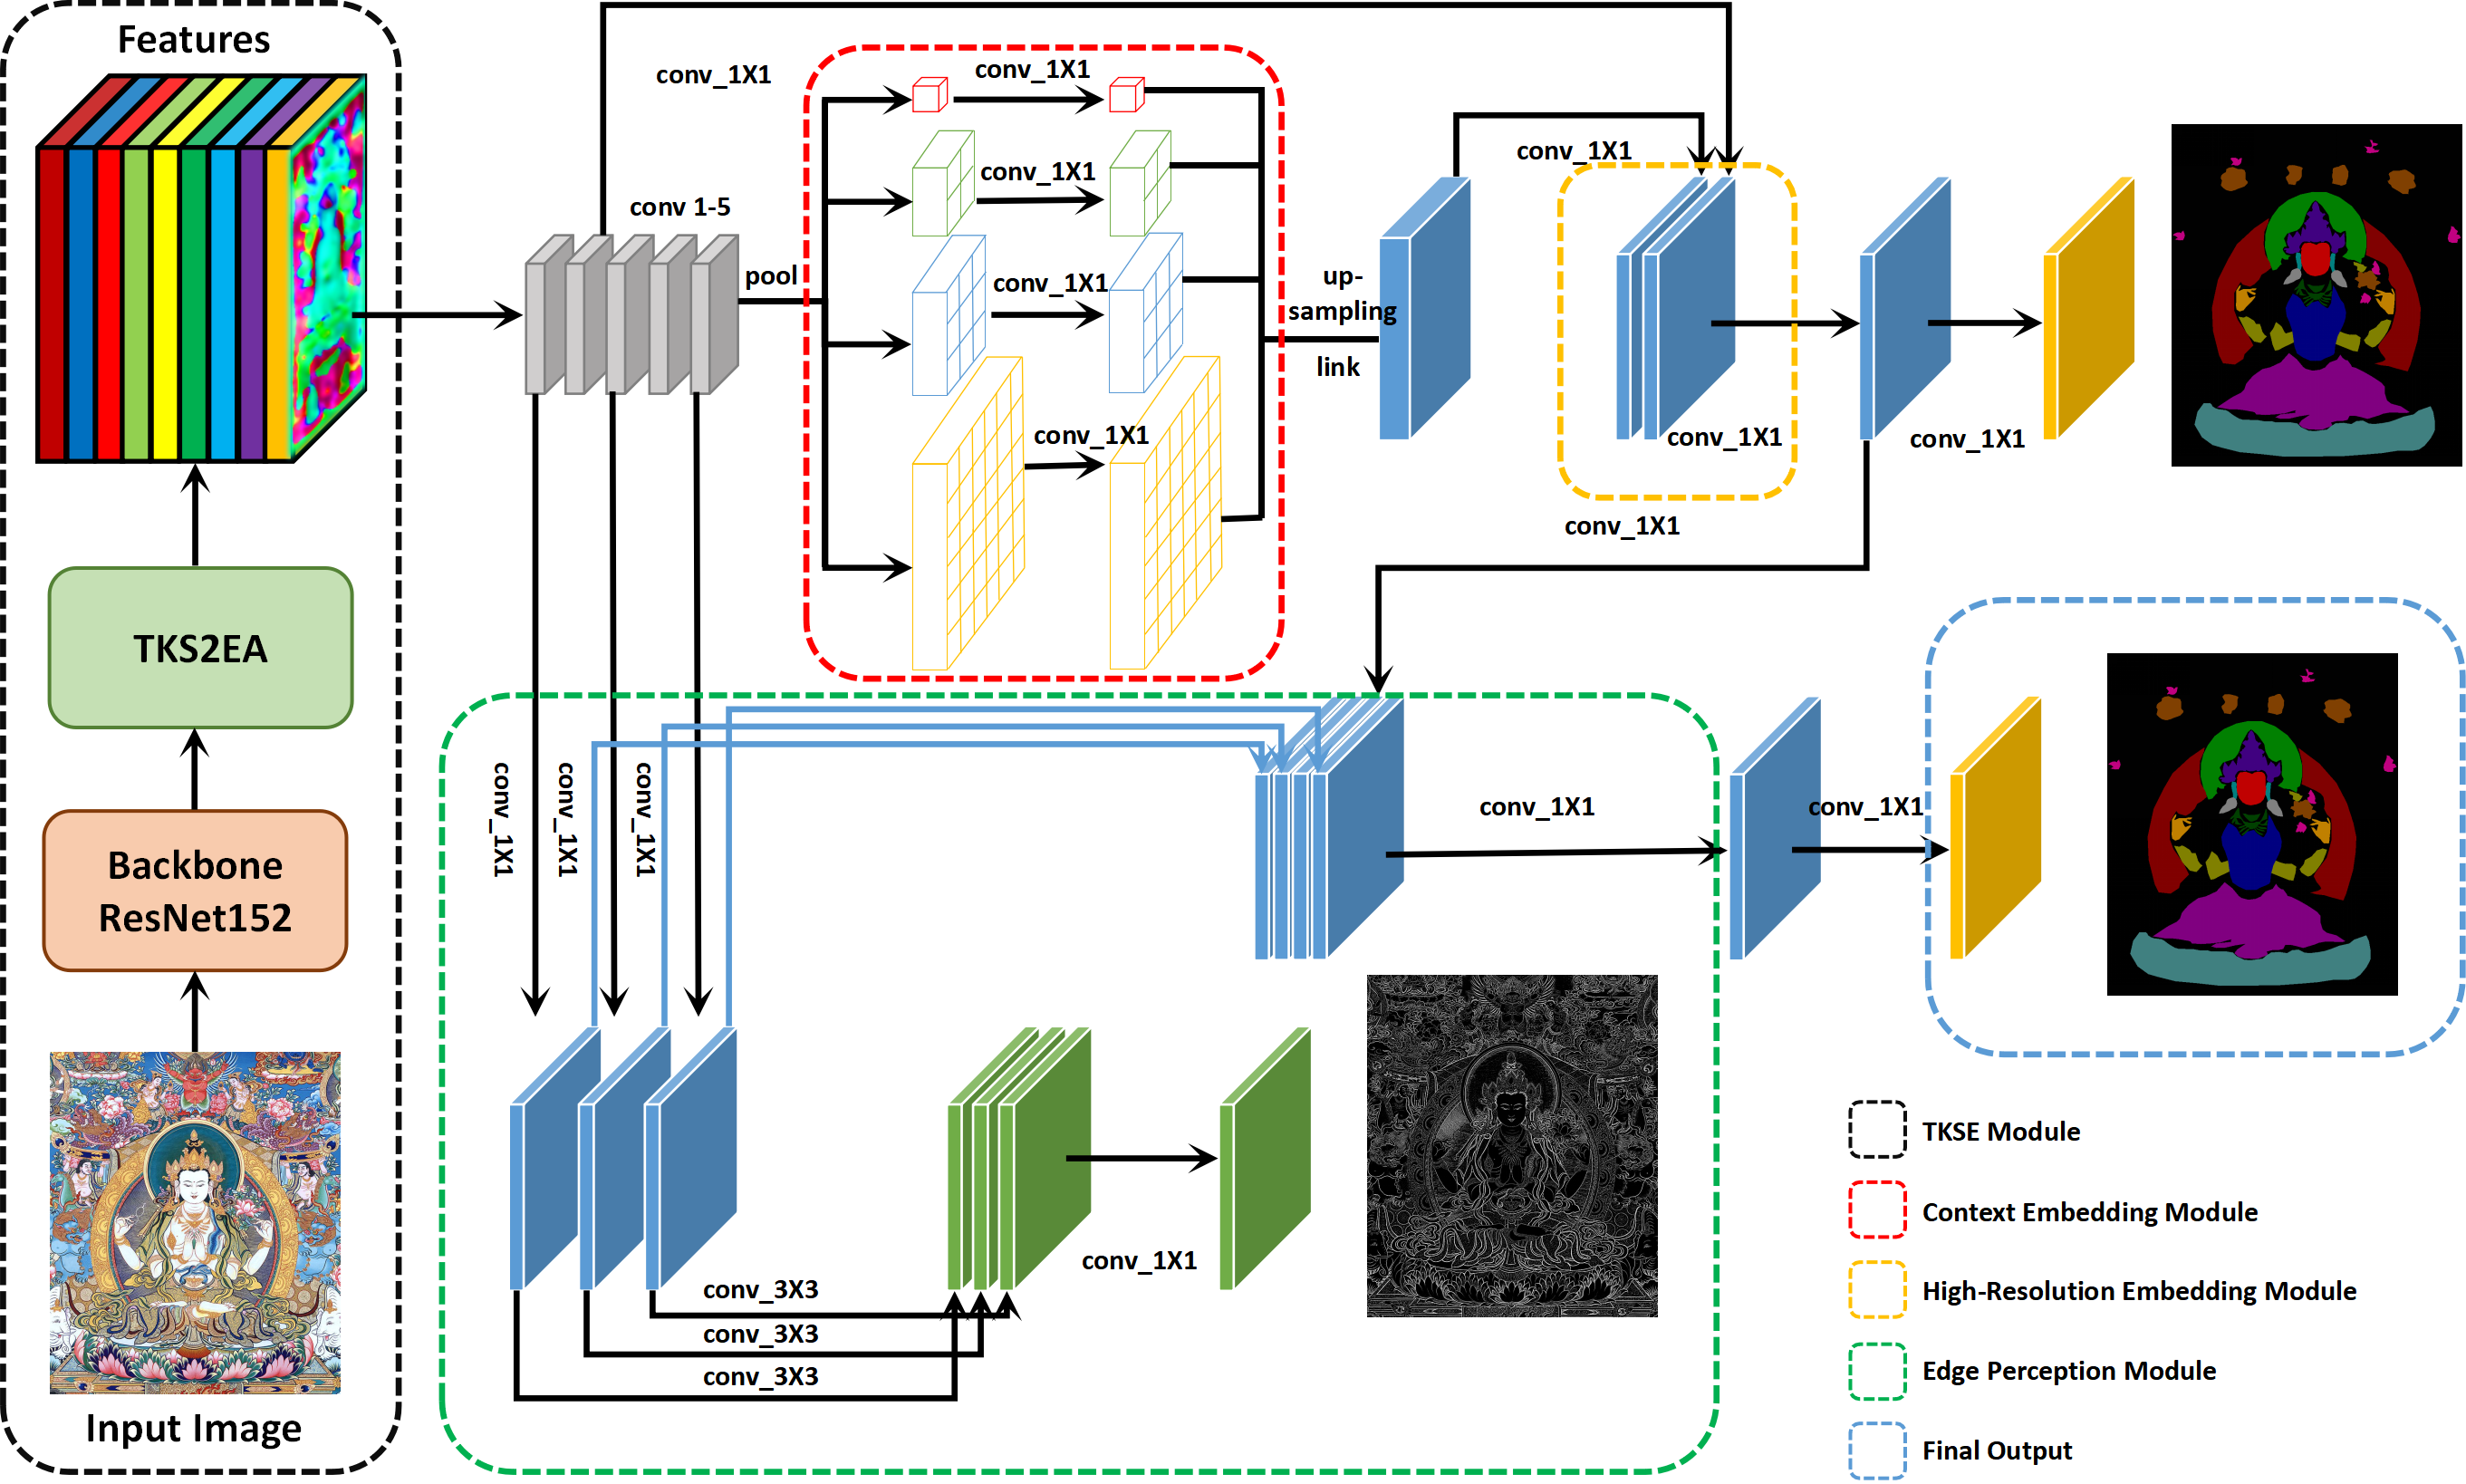
\includegraphics[width=1\linewidth]{fig4.png}}
	\caption{TKSS module.}
	\label{fig4}
\end{figure}
The network architecture comprises four core components: An attention mechanism module for enhanced feature representation; A context embedding module for capturing global semantic information; A high-resolution embedding module for preserving local detail features; and An edge-aware module for improving boundary segmentation accuracy. The network employs ResNet 152 as the backbone feature extractor to achieve end-to-end semantic segmentation optimization. This multi-scale feature fusion design significantly improves segmentation performance, particularly in maintaining fine details and boundary accuracy in complex scenarios. While the TKS2EA attention mechanism module will be detailed in the next subsection, the other three modules are described below.

Context Embedding Module. To address the challenge of distinguishing fine-grained categories in Thangka images (e.g., left/right hands, decorative patterns), this module incorporates pyramid pooling (PPM), inspired by PSPNet \cite{b32}, to capture global context. Specifically, multi-scale pooling (1×1, 2×2, 3×3, 6×6) is applied to the deep features from ResNet 152, generating contextual features with varying receptive fields. These features are upsampled, concatenated, and fused through 1×1 convolution to form a semantic representation with global priors, providing category-discriminative cues for subsequent segmentation.

High-Resolution Embedding Module. To mitigate detail loss in small object segmentation (e.g., jewelry, topknots), this module fuses shallow high-resolution features (conv2) with deep semantic features. First, the global features output by the context module are upsampled 4× and reduced in dimension via 1×1 convolution before being concatenated with local features. The fused features are then refined through two additional 1×1 convolutions. The final output preserves both high-resolution spatial information and high-level semantics, significantly improving segmentation accuracy for small objects.

Edge-Aware Module. To sharpen segmentation boundaries, this module adopts a multi-scale edge detection strategy. Edge response maps are generated by applying 1×1 convolutions to the conv2, conv3, and conv4 layers, respectively, and then fused to obtain multi-scale edge features. These features are upsampled and concatenated with the output of the high-resolution module before being processed by a final 1×1 convolution to produce edge-enhanced segmentation results, effectively improving the clarity of object contours. 

\subsubsection{TKS2EA Module}
The TKS2EA module is inspired by HR-NAS \cite{b33} and improved based on the SENet \cite{b34} architecture, incorporating dual mechanisms of spatial attention and channel attention to accomplish Thangka Buddha region recognition. As shown in Fig.~\ref{fig5}, this section details the four key components of the proposed TKS2EA attention mechanism module.
\begin{figure}[htbp]
	\centerline{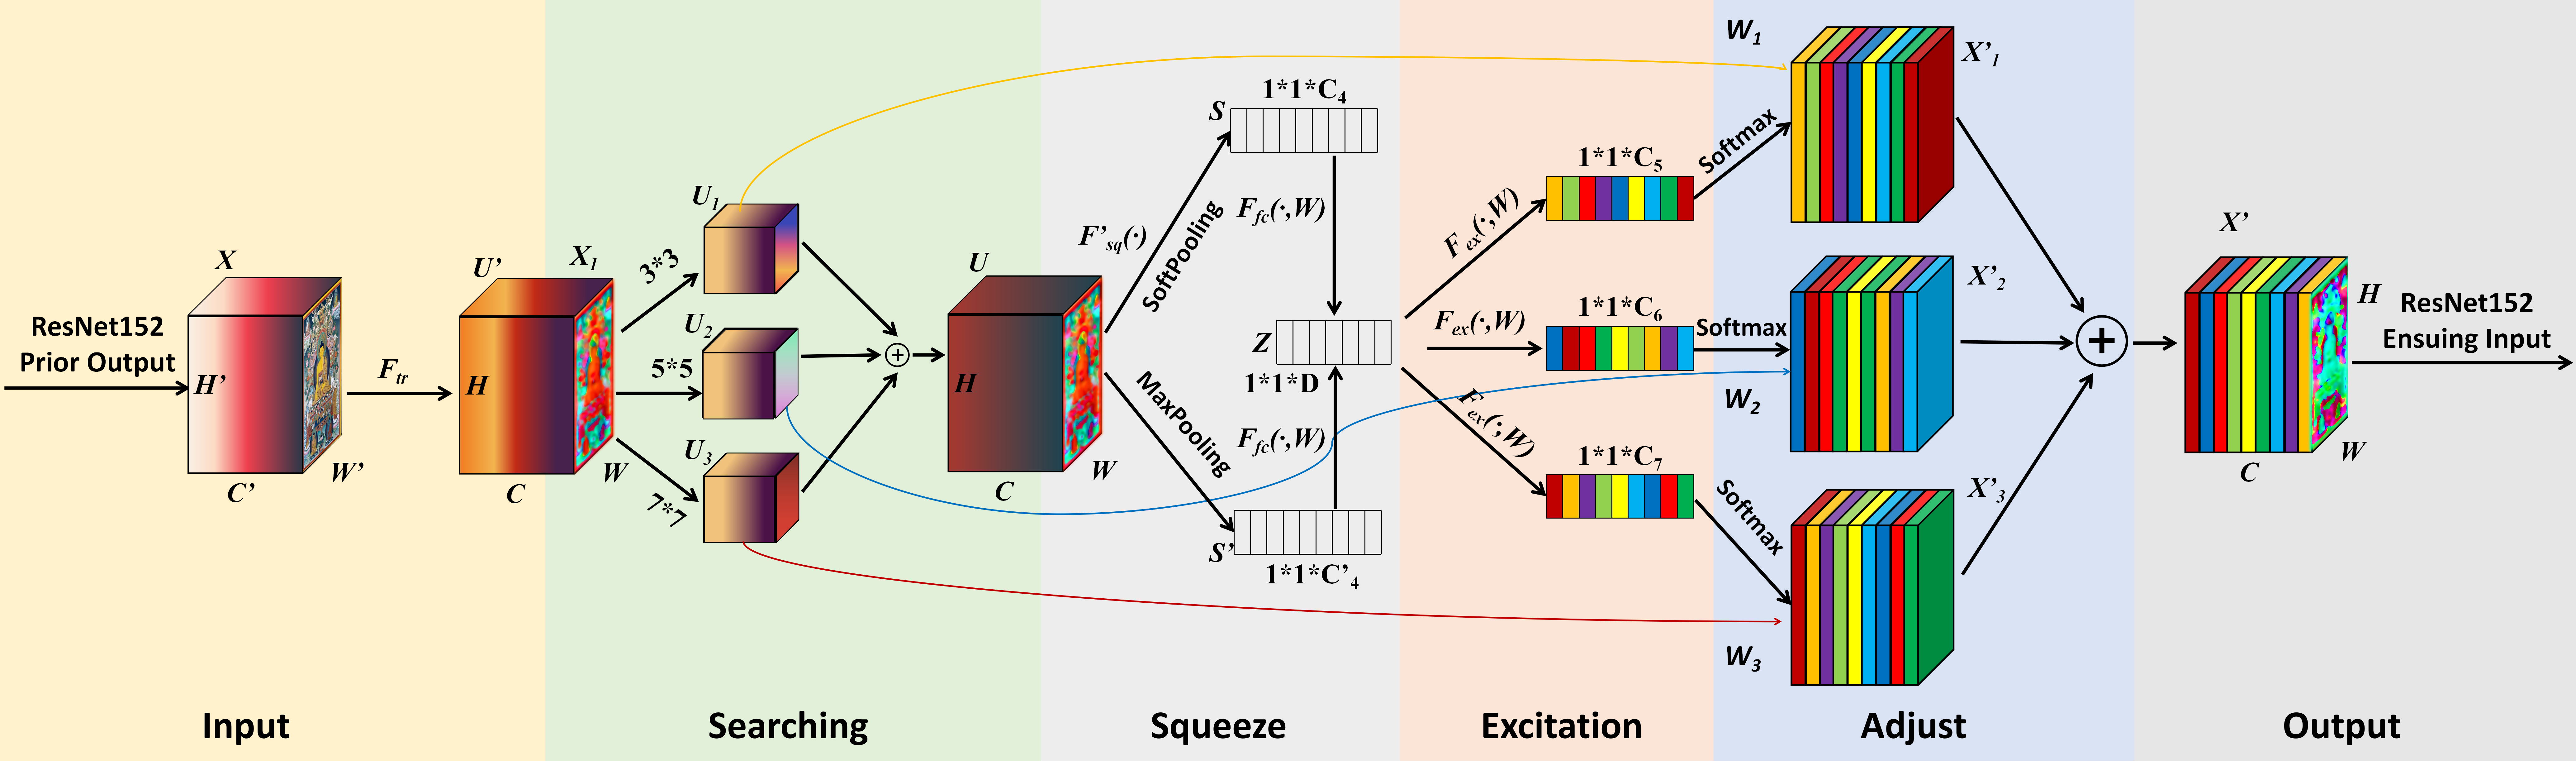
\includegraphics[width=1\linewidth]{fig5.png}}
	\caption{TKS2EA module.}
	\label{fig5}
\end{figure}

\textbf{Search Operation of TKS2EA. }The search operation processes input image $ U' $ with different convolutional kernels following customized rules:  

A 3×3 kernel convolves the main Buddha region to obtain $ {U_1} $  

A 5×5 kernel processes Buddha-related accessory regions to yield $ {U_2} $  

A 7×7 kernel handles background areas to generate $ {U_3} $  

The final feature map U is obtained through element-wise summation:  
\begin{equation}
	U = {U_1} + {U_2} + {U_3}
	\label{eq5}
\end{equation}
\textbf{Squeeze Operation of TKS2EA. }The convolutional output $ X $ from ResNet 152 undergoes multiple convolutional operations and re-weighting to obtain feature map U, where spatial importance is represented through weight values. For feature extraction, $ U $ serves as input to the compression operation through pooling. The original feature block dimensions (H×W×C) are thus compressed to 1×1×C, achieving global receptive field coverage through dimensionality reduction.

To derive channel-wise weights, soft pooling first computes feature value weights as shown in Eq.\eqref{eq6}, where $ U \in\mathbb{R}{^{H \times W \times C}} $ denotes the convolved feature block from preceding layers, and $ x $ represents feature values:  
\begin{equation}
	{w_i}=\frac{{{e^{{x_i}}}}}{{\sum\limits_{j \in U} {{e^{{x_j}}}} }}
	\label{eq6}
\end{equation}
These weights are multiplied with corresponding features and aggregated via Eq.\eqref{eq7}, yielding a 1×1×C feature block: 
\begin{equation}
	{y_c}=x'=\sum\limits_{i \in U} {{w_i}*{x_i}}
	\label{eq7}
\end{equation}
Subsequent fusion and compression of two 1×1×\textbf{C} feature maps establishes inter-channel dependencies through fully-connected (FC) layers and activation functions (Eq.\eqref{eq8}). This eliminates low-weight features to produce a 1×1×$ D $  feature map $ Z $ ($ C>D $):  
\begin{equation}
	z={F_{fc}}(s)=\xi (\beta (Ws))
	\label{eq8}
\end{equation}
\begin{equation}
	d=max(C/r,L)
	\label{eq9}
\end{equation}
Here, $ Z $ has dimensions 1×1×$ D $, $ \xi $ is the Leaky ReLU activation function, $ \beta $ represents batch standardized BN, $ W \in\mathbb{R}{^{1 \times d \times C}} $, $ d $ in Eq.\eqref{eq9} represents the fully connected feature dimension, $ L $ is set to 32, $ r $ is the scaling parameter, and $ r=16 $ is set here.

\textbf{Excitation Operation of TKS2EA.} A schematic diagram of the TKS2EA block embedded in ResNet 152 is shown in Fig.~\ref{fig6}. The dimension of the feature map $ Z $ is renormalized from 1×1×$ D $ to 1×1×$ C $. After receiving the compressed output feature map of size 1×1×C, the TKS2EA excitation operation sequentially and alternately introduces two fully connected layers and two activation functions to predict the importance of each channel in $ C $. The weights representing the importance of different channels are then applied to the corresponding channels of the previous feature block for subsequent operations.
\begin{figure}[htbp]
	\centerline{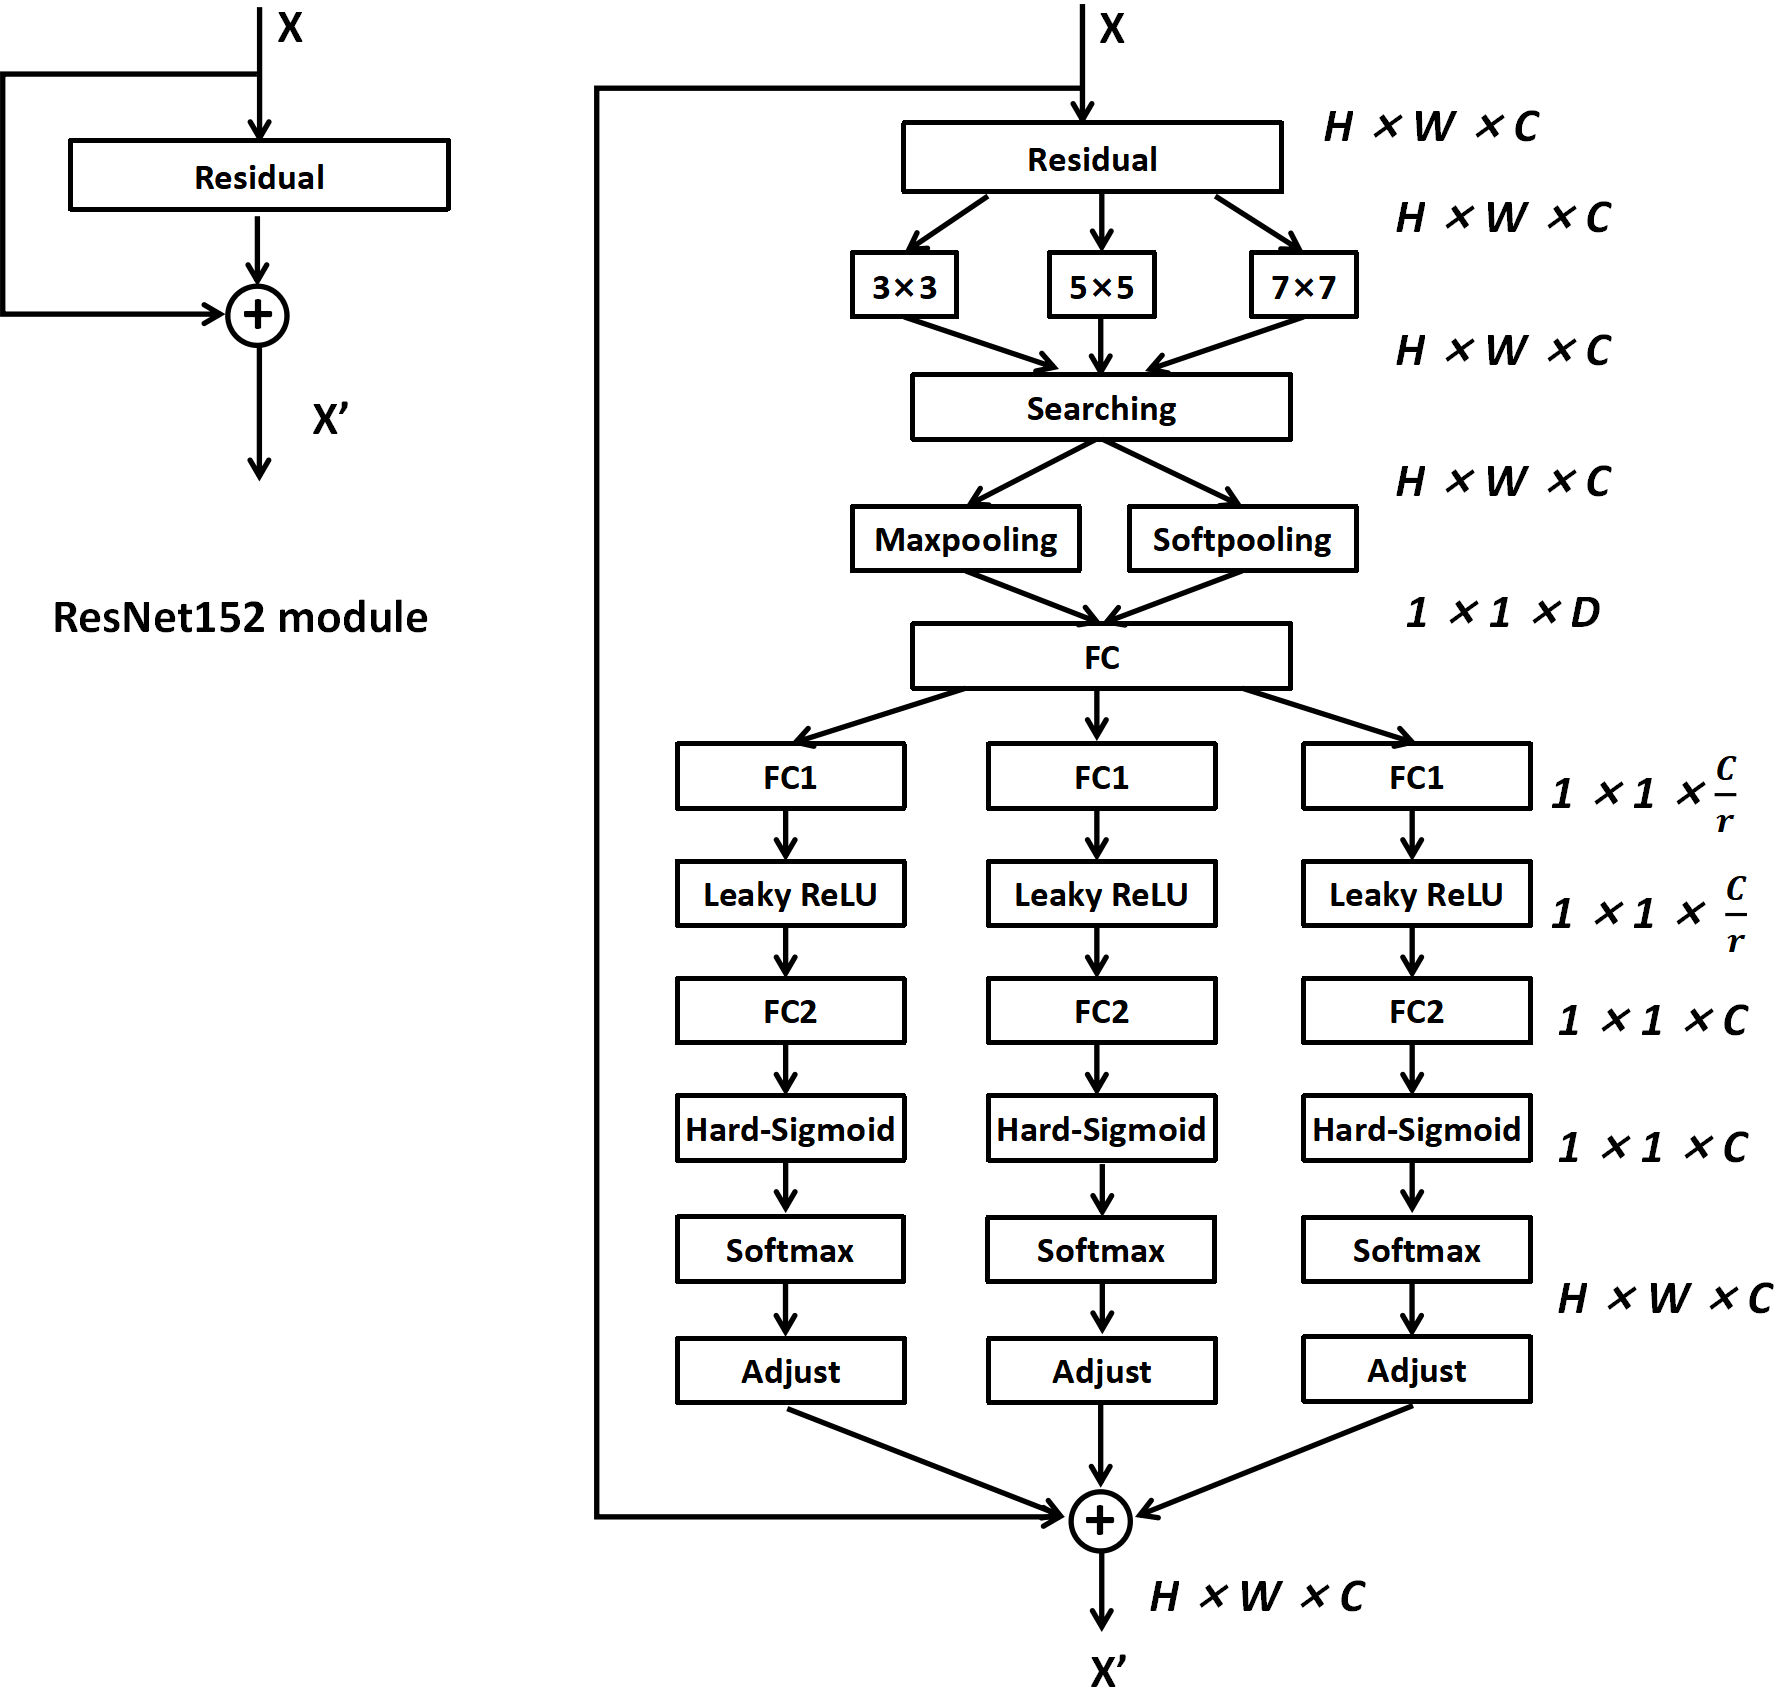
\includegraphics[width=0.65\linewidth]{fig6.png}}
	\caption{Flowchart of TKS2EA embedded in ResNet 152.}
	\label{fig6}
\end{figure}
The operational flow of each layer in Figure1 is as follows:  

The process of the TKS2EA excitation operation is shown in Eq.\eqref{eq10}, where y is the result from Eq.\eqref{eq7}, $ y \in {\mathbb{R}^{1 \times 1 \times C}} $. Here, $ y $ is first multiplied by the parameter $ {W_1} $ in the first fully connected layer, $ {W_1} \in {\mathbb{R}^{{\raise0.7ex\hbox{$C$} \!\mathord{\left/
				{\vphantom {C r}}\right.\kern-\nulldelimiterspace}
			\!\lower0.7ex\hbox{$r$}} \times C}} $, where $ r $ is the scaling parameter, resulting in $ {W_1}y \in {\mathbb{R}^{1 \times 1 \times {\raise0.7ex\hbox{$C$} \!\mathord{\left/
				{\vphantom {C r}}\right.\kern-\nulldelimiterspace}
			\!\lower0.7ex\hbox{$r$}}}} $.  
\begin{equation}
	{\rm{s}} = {F_{ex}}(y,W) = \phi (g(y,W)) = \phi ({W_2}\xi ({W_1}y))
	\label{eq10}
\end{equation}
To address the above issues, during the excitation operation, TKS2EA uses the Leaky ReLU activation function after the first fully connected layer, followed by the second fully connected layer and the Hard-Sigmoid activation function.  
In Eq.\eqref{eq10}, $ \xi $ represents the Leaky ReLU activation function. After activation by Leaky ReLU, the dimension remains unchanged, so $ \xi ({W_1}y) \in {\mathbb{R}^{1 \times 1 \times {\raise0.7ex\hbox{$C$} \!\mathord{\left/
				{\vphantom {C r}}\right.\kern-\nulldelimiterspace}
			\!\lower0.7ex\hbox{$r$}}}} $. This is then multiplied by $ {W_2} $, $ {W_2} \in {\mathbb{R}^{C \times {\raise0.7ex\hbox{$C$} \!\mathord{\left/
				{\vphantom {C r}}\right.\kern-\nulldelimiterspace}
			\!\lower0.7ex\hbox{$r$}}}} $, resulting in a dimension of 1×1×$ C $ after the second fully connected layer, $ {W_2}\xi ({W_1}y) $. Finally, another activation function $ \varphi $ is applied, where $ \varphi $ is the Hard-Sigmoid activation function, aimed at correcting the Leaky ReLU activation function to accelerate the convergence of the network model. After Hard-Sigmoid activation, the dimension remains unchanged, and the final output $ s $, $s \in {\mathbb{R}^{1 \times 1 \times C}} $, is obtained.  

\textbf{Adjust Operation of TKS2EA. }The three feature maps of size 1×1×C output from the excitation operation undergo feature selection, and the weights of each convolutional kernel are calculated using Softmax and applied to the weighting operation. These weights are treated as importance parameters for the feature channels, describing the weight magnitude of each 1×1×1 feature block in the feature block $ U $. Next, these weights are applied to the original features before compression through channel-wise multiplication, thereby rescaling the weights of the original features along the channel dimension. The weighted sum of the three feature blocks yields $ X’ $, as shown in Eq.\eqref{eq11}, which serves as the input for the ResNet 152 model for subsequent operations and computations. This method enables the model to achieve better performance through end-to-end training.
\begin{equation}
	{X'} = {X'}_1 + {X'}_2 + {X'}_3
	\label{eq11}
\end{equation}
\subsection{Feature Fusion Module}
Finally, TKSegDiff employs the Feature Fusion Module (FFM) to integrate contextual features from both the TKSS-guided segmentation and the metric-constrained reverse denoising stages, predicting the final generated Thangka image through a decision head. The FFM utilizes global contextual relationships as prior knowledge to refine local contextual features, producing fused representations that capture both global coherence and local details. As illustrated in Fig.~\ref{fig3}, the FFM consists of a spatial feature transformation block followed by two 3×3 convolutional layers, each accompanied by batch normalization and ReLU activation. The former adjusts feature distributions, while the latter ensures smoothness. The fused features are then fed into the Decision Head ($ D_H $) to predict the final Thangka image $ x' $ as formulated in Eq.\eqref{eq12}, where $ D_H $ comprises a 1×1 convolutional layer and a Sigmoid activation function. 
\begin{equation}
	\tilde x = {D_H}(FFM({f_t},{f_d}))
	\label{eq12}
\end{equation}
$ D_H $ is a decision head composed of 1×1 convolutional layers and Sigmoid function activation operations.
\subsection{Loss Function}
The TKSegDiff model adopts a weighted multi task loss form:
\begin{equation}
	\mathcal{L}_{\mathrm{total}}=\lambda_1\mathcal{L}_{\mathrm{diffusion}}+\lambda_2\mathcal{L}_{\text{segmentation}}+\lambda_3\mathcal{L}_{\mathrm{cultural}}+\lambda_4\mathcal{L}_{\mathrm{fusion}}
	\label{eq13}
\end{equation}
This paper employs dynamic weight adjustment, where $ {\lambda _1} $ is fixed at 1.0; $ {\lambda _2} $ is set to 0.5 and dynamically scaled each epoch based on the validation set mIoU; $ {\lambda _3} $ is initially set to 0.3 and linearly increases to 0.5 during the first 10\% of training steps; $ {\lambda _4} $ is set to 0.2 and triggered when Lfusion exceeds a threshold. Here, Ldiffusion represents the basic diffusion model loss, which adopts a Hybrid Loss combining noise prediction and image reconstruction, expressed as:
\begin{equation}
	\mathcal{L}_{\mathrm{diffusion}}=\mathbb{E}_{t,\epsilon}\left[\|\epsilon-\epsilon_\theta(\mathbf{x}_t,t,\mathbf{T}_m)\|_1\right]+\gamma\cdot\mathrm{LPIPS}(\mathbf{x}_0,\hat{\mathbf{x}}_0)
	\label{eq14}
\end{equation}
The first term in the equation represents the $ L_1 $ noise prediction loss, while the second term denotes the LPIPS perceptual loss (with weight $\gamma $=0.8) for preserving visual quality, where Tm represents the Iconometric Token condition. $L_{segmentation}$ constitutes the semantic segmentation loss associated with the supervision signal of the TKSS module. To address Thangka's characteristic of containing numerous small objects, we employ a Focal-Dice Loss:
\begin{equation}
	\mathcal{L}_{\mathrm{segmentation}}=\alpha\cdot\mathcal{L}_{\mathrm{Focal}}+(1-\alpha)\cdot\mathcal{L}_{\mathrm{Dice}}
	\label{eq15}
\end{equation}
The Focal Loss is employed to address class imbalance issues, while the Dice Loss is utilized to enhance segmentation performance for small objects.
\begin{equation}
	\mathcal{L}_{\mathrm{Focal}}=-\sum_c(1-p_c)^\beta\cdot y_c\log(p_c),\quad\beta=2
	\label{eq16}
\end{equation}
\begin{equation}
	\mathcal{L}_{\mathrm{Dice}}=1-\frac{2\sum p_cy_c+\epsilon}{\sum p_c+\sum y_c+\epsilon}
	\label{eq17}
\end{equation}
The cultural feature loss Lcultural is designed to ensure the generated Thangka images strictly adhere to cultural constraints. First, the global proportion loss $\mathcal{L}_{\text{metric}}$ enforces the geometric proportion rules specified in the 'The Sacred Canon of Measurements for Thangka Buddha Figures'. This paper employs a pre-trained keypoint detection model to extract anatomical keypoints from both generated and authentic Thangka images, then calculates the error in relative distances between corresponding keypoints:
\begin{equation}
	{\mathcal{L}_{{\rm{metric}}}} = \sum\limits_{i,j} {\left\| {\frac{{\left\| {{\bf{k}}_i^{{\rm{gen}}} - {\bf{k}}_j^{{\rm{gen}}}} \right\|}}{{\left\| {{\bf{k}}_a^{{\rm{gen}}} - {\bf{k}}_b^{{\rm{gen}}}} \right\|}} - \frac{{\left\| {{\bf{k}}_i^{{\rm{real}}} - {\bf{k}}_j^{{\rm{real}}}} \right\|}}{{\left\| {{\bf{k}}_a^{{\rm{real}}} - {\bf{k}}_b^{{\rm{real}}}} \right\|}}} \right\|} 
	\label{eq18}
\end{equation}
Here, $\textbf{k}_*^{gen}$ represents the detected keypoints in the generated image, while $\textbf{k}_*^{real}$ denotes the keypoints in authentic Thangka paintings. The denominator term indicates the reference distance, and the numerator represents the measured distance. This loss function is relatively complex, as illustrated by the following example: 
Example: If 'The Sacred Canon of Measurements for Thangka Buddha Figures' specifies that "the total height of a standing Buddha statue = 4 × head height," the loss penalizes cases where $$\frac{\|\mathbf{k}_{\text{ushnisha}}-\mathbf{k}_{\text{feet}}\|}{4\|\mathbf{k}_{\text{ushnisha}}-\mathbf{k}_{\text{chin}}\|} \neq 1$$ in the generated image.
Additionally, the symbolic discriminative loss \(\mathcal{L}_{\text{symbol}}\) enforces the correct representation of religious symbols (e.g., ritual objects and hand gestures). This paper introduces a Thangka symbol classifier \(C_{\text{symbol}}\), which compares the probability distributions of symbols between generated and real images:
\begin{equation}
	\mathcal{L}_{\mathrm{symbol}}=D_{\mathrm{KL}}(C_{\mathrm{symbol}}(\mathbf{x}_{\mathrm{real}})\|C_{\mathrm{symbol}}(\mathbf{x}_{\mathrm{gen}}))
	\label{eq19}
\end{equation}
The final cultural loss is formulated as a weighted sum of the three-level losses:
\begin{equation}
	\mathcal{L}_{\mathrm{cultural}}=\lambda_{\mathrm{metric}}\mathcal{L}_{\mathrm{metric}}+\lambda_{\mathrm{symbol}}\mathcal{L}_{\mathrm{symbol}}
	\label{eq20}
\end{equation}
In the initial training phase, greater emphasis is placed on proportional accuracy with $ {\lambda _{metric}} $=0.6, while in later stages the focus shifts to symbolic correctness with $ {\lambda _{symbol}} $=0.4. The feature fusion loss $ L_{fusion} $ is employed for quality control in the feature fusion module, utilizing contrastive learning loss to minimize the distance between generated features and authentic features:
\begin{equation}
	\mathcal{L}_{\mathrm{fusion}}=-\operatorname{log}\frac{\operatorname{exp}(\operatorname{sim}(\mathbf{h}_{\mathrm{gen}},\mathbf{h}_{\mathrm{real}})/\tau)}{\sum_{i=1}^{N}\operatorname{exp}(\operatorname{sim}(\mathbf{h}_{\mathrm{gen}},\mathbf{h}_{\mathrm{neg}_{i}}})/\tau)
	\label{eq21}
\end{equation}
where $ \textbf{h}_{gen} $ represents the generated features output by the fusion module, and $\tau$ denotes the temperature coefficient ($\tau$=0.07 in our experiments). 
\section{Experiments and Analysis}
\subsection{Dataset and Baselines}
\textbf{Dataset.} Since no publicly available dataset with annotations exists for Thangka image generation research, we constructed the TK-10K dataset, comprising 10,000 high-resolution Thangka images (resolution $ \ge $ 1024×1024).
\begin{figure}[htbp]
	\centerline{\includegraphics[width=0.7\linewidth]{fig7.png}}
	\caption{Dataset visualization.}
	\label{fig7}
\end{figure}
Each image is annotated with pixel-level semantic segmentation labels across 20 categories, as shown in Fig.~\ref{fig7}, including main deity, ritual objects, cloud patterns, and halos. Additionally, under the guidance of Thangka artists, we labeled keypoints based on 'The Sacred Canon of Measurements for Thangka Buddha Figures', totaling 12 anatomical points and 8 ritual object points.

\textbf{Baseline Methods.} We selected several open-source models for comparison: SPADE\cite{b14} (2019), SMAC-CGAN\cite{b15} (2023), Karlo\cite{b21} (2024), FLUX.1\cite{b22} (2024), Stable Diffusion 3\cite{b24} (2025), and BAGEL\cite{b23} (2025). Each model was trained using Thangka images paired with textual descriptions for fair evaluation.
\subsection{Experimental Setup and Evaluation Metrics}
$ Experimental Setup. $ In this experiment, the CPU is Intel(R) Xeon(R) Gold 6226 CPU @ 2.70GHz, the 2 GPU is NVIDIA GeForce RTX 4090 with 24 GB of Graphics memory. The algorithm is implemented by PyTorch1.12, using CUDA 11.6 to operation acceleration. 

$ Quantitative Analysis. $ We employ objective evaluation metrics including FID \cite{b35} and PSNR \cite{b36} to assess generation quality, along with the structural accuracy metric mIoU \cite{b37} to measure the discrepancy between generated and ground-truth segmentation maps.  

$ Qualitative Analysis. $ We adopt the Average Human Ranking (AHR) \cite{b38} as a subjective evaluation metric for assessing the quality of generated Thangka images. The AHR implementation in this study is designed as follows:  

During the ranking process for each generated result, participants are asked: 'Which of the following Thangka images appears least AI-generated? Please rank the images based on your judgment.' The study involves 30 evaluators: 10 non-art students, 10 art students, and 10 professional Thangka painters with at least five years of experience. From each of the N comparative methods, S randomly selected generated Thangka images are sampled, resulting in S × (N + 1) images in total (including our method). Participants rank these S × (N + 1) results, with rankings divided into three tiers (A, B, C, where A > B > C). Each tier accommodates N/3 results, and participants first group the generated images into three categories before assigning rankings within each group: A $ \in $[1, N/3], B$ \in $[N/3 + 1, 2N/3], and C$ \in $ [2N/3 + 1, N]. In this study, $ S=6 $ and $ N=6 $. The final AHR score is derived from the average ranking across all evaluations.
\subsection{Ablation Study}
To validate the effectiveness of each module, we conducted ablation experiments, with the results presented in Table.~\ref{tab1}. It can be seen that if any module is missing, the performance of the model will decrease. This indicates that the three modules of TKSegDiff are complementary and indispensable. Additionally, the sketch extraction results of No.1-No.4 are shown in Fig.~\ref{fig8}.
\begin{table}[htbp]\tiny
	\begin{center}
		\caption{Conduct ablation study on the effectiveness of the proposed three modules on TK-10K datasets.}
		\label{tab1}
		\setlength\tabcolsep{0.5mm}{
			\begin{tabular}{c|ccc|c|c|c|c|c|c}
				\hline
				\cellcolor[HTML]{FFFFFF}Num & Canon Token & TKSS & FFM & Time/hours & FLOPs/G & FID↓better     & PSNR↓better    & mIoU↑better      & AHR↓better    \\ \hline
				No.1                        & $\surd $           & -    & -   & 106.6      & 3037.1  & 56.47          & 11.39          & 46.38\%          & 3.33          \\
				No.2                        & -           & $\surd $    & -   & 135.8      & 3159.7  & 73.26          & 15.74          & 36.92\%          & 3.33          \\
				No.3                        & $\surd $           & $\surd $    & -   & 156.6      & 3462.4  & 32.43          & 23.75          & 74.33\%          & 2.33          \\
				No.4                        & $\surd $           & $\surd $    & $\surd $   & 163.8      & 3579.3  & \textbf{29.83} & \textbf{27.41} & \textbf{85.36\%} & \textbf{1.00} \\ \hline
			\end{tabular}
		}
	\end{center}
\end{table}
\begin{figure}[htbp]
	\centerline{\includegraphics[width=0.8\linewidth]{fig8.png}}
	\caption{Ablation study. We examine the improvement in generative  performance brought by each individual module through incremental addition to the framework.}
	\label{fig8}
\end{figure}
The experimental results demonstrate that removing the Iconometric tokens leads to disproportional generation of Buddha figures, while eliminating the TKSS module causes a noticeable decline in mIoU. Furthermore, the removal of feature fusion results in a significant increase in FID score.
\subsection{Comparison with State-of-the-arts}
\textbf{Quantitative results.} To comprehensively evaluate the performance advantages of the TKSegDiff model, we conducted systematic training and testing on the self-built Thangka dataset TK-10K under standard experimental conditions (PyTorch 1.12 + CUDA 11.6, dual NVIDIA GeForce RTX 4090 GPUs). As shown in Table.~\ref{tab2}. By training on the TK-10K dataset, our method achieved subjective evaluation scores of 1.33 for AHR, and an objective evaluation score of 29.83 for FID, 27.41 for PSNR and 85.36\% for mIoU. The quantitative analysis results demonstrate that TKSegDiff significantly outperforms existing comparative methods across all evaluation metrics, exhibiting superior performance advantages.
\begin{table}[htbp]\tiny
	\begin{center}
		\caption{Comparative experimental results of The quantitative analysis.}
		\label{tab2}
		\setlength\tabcolsep{0.5mm}{
			\begin{tabular}{ccccccc}
				\hline
				Methods                                                             & Time/hours     & FLOPs/G         & FID↓better     & PSNR↓better    & mIoU↑better      & AHR↓better    \\ \hline
				\begin{tabular}[c]{@{}c@{}}SPADE\cite{b14}\\ (2019)\end{tabular}              & 78.6           & 1286.7          & 58.55          & 13.65          & 41.33\%          & 6.67          \\ \hline
				\begin{tabular}[c]{@{}c@{}}SMAC-CGAN\cite{b15}\\ (2023)\end{tabular}          & 56.4           & 963.9           & 53.26          & 17.33          & 43.84\%          & 5.33          \\ \hline
				\begin{tabular}[c]{@{}c@{}}Karlo\cite{b21}\\ (2024)\end{tabular}              & 247.6          & 4537.6          & 43.64          & 18.91          & 46.01\%          & 4.33          \\ \hline
				\begin{tabular}[c]{@{}c@{}}FLUX.1\cite{b22}\\ (2024)\end{tabular}             & 258.6          & 4739.3          & 41.11          & 19.28          & 63.49\%          & 3.67          \\ \hline
				\begin{tabular}[c]{@{}c@{}}Stable Diffusion 3\cite{b24}\\ (2025)\end{tabular} & 165.4          & 3768.1          & 42.36          & 18.68          & 61.27\%          & 3.00          \\ \hline
				\begin{tabular}[c]{@{}c@{}}BAGEL\cite{b23}\\ (2025)\end{tabular}              & 179.3          & 4535.8          & 39.15          & 20.54          & 70.75\%          & 3.67          \\ \hline
				\textbf{\begin{tabular}[c]{@{}c@{}}TKSegDiff\\ (Ours)\end{tabular}} & \textbf{163.8} & \textbf{3579.3} & \textbf{29.83} & \textbf{27.41} & \textbf{85.36\%} & \textbf{1.33} \\ \hline
			\end{tabular}
		}
	\end{center}
\end{table}

\textbf{Qualitative results.} To further validate the generation performance of the TKSegDiff model, we conducted an in-depth qualitative analysis. As shown in Fig.~\ref{fig9}, the visual comparison results demonstrate that our proposed TKSegDiff model exhibits significant advantages over existing methods in Thangka image generation tasks. Specifically, the model demonstrates the ability to: 1) accurately capture the distinctive artistic style and religious elements of Thangka; 2) maintain high consistency in image details; 3) generate color transitions with authentic texture. Particularly noteworthy is that the Thangka images generated by the model achieve near-authentic levels in terms of texture refinement, compositional integrity, and artistic expression, which fully demonstrates TKSegDiff's outstanding capabilities in the field of cultural artwork generation.
\begin{figure}[htbp]
	\centerline{\includegraphics[width=1\linewidth]{fig9.png}}
	\caption{Comparative Experimental Results of The Qualitative Analysis.}
	\label{fig9}
\end{figure}
\section{CONCLUSIONS}
\textbf{Conclusions:} This paper proposes a semantic segmentation-guided diffusion model for Thangka generation (TKSegDiff), addressing the structural distortion, semantic confusion, and global incoherence prevalent in conventional generation methods. By encoding the religious canons from the 'Iconometric Sutra' into learnable dynamic embeddings and integrating them via cross-attention mechanisms, our approach effectively constrains the generation process to ensure compliance with traditional standards in key elements such as Buddha proportions and ritual object placement. Furthermore, the proposed TKS2EA-enhanced segmentation network significantly improves fine-grained semantic segmentation accuracy (85.36\% mIoU), while the feature fusion module optimizes global style consistency. Experimental results demonstrate that TKSegDiff outperforms Stable Diffusion by 29.58\% and BAGEL by 23.80\% in FID metrics, achieving a 75\% approval rate in blind evaluations by cultural experts, thereby validating its practical value for Thangka digital preservation.

\textbf{Limitations:} Despite its strong performance in Thangka generation, the current method has the following limitations: The model primarily targets specific Thangka styles (e.g., Menri and Karma Gadri), while its adaptability to other styles (e.g., black or gold Thangka) requires further validation. The generation process relies on static semantic maps for guidance, lacking interactive capabilities for real-time user adjustments of fine details.

\textbf{Future: } Building on this study, future directions include: Reducing dependence on finely annotated data by leveraging unsupervised or semi-supervised methods to enhance model generalization. Incorporating style transfer techniques to enable on-demand generation of Thangka across diverse styles and color schemes.  
\section{Acknowledgment}
This work is supported by the Central guidance of local scientific and technological development funds in Qinghai Province (NO. 2024ZY050).

\section{Author contributions statement}

Fubo Wang conceived the experiments,  Shengling Geng conducted the experiments.
%%, Wanyi Zhao, Zeyu Jia and Mingcong Dang analysed the results. All authors reviewed the manuscript. 

\section{Additional information}

\textbf{Competing interests}. The authors declare no competing interests. \textbf{Data availability}. The datasets generated and analysed during the current study are not publicly available due to intellectual property rights concerns related to Tibetan painting artisans, for which only our team has been authorized to use, but are available from the corresponding author upon reasonable request.

\begin{thebibliography}{00}
	\bibitem{b1} Ma Y, Liu Y, Xie Q, et al. A Tibetan Thangka data set and relative tasks[J]. Image and Vision Computing, 2021, 108: 104125.
	\bibitem{b2} Bhaumik G, Govil M C. Conserving Thangka-A technical approach unto the preservation of Buddhist Thangka through automation[J]. Digital Applications in Archaeology and Cultural Heritage, 2020, 18: e00149.
	\bibitem{b3} Hu W, Ye Y, Zeng F, et al. A new method of Thangka image inpainting quality assessment[J]. Journal of Visual Communication and Image Representation, 2019, 59: 292-299.
	\bibitem{b4} Yang Q, Yang J, Ni S, et al. Research on the classification model of Thangka subjects based on efficient PatchEmbed[C]//2024 International Joint Conference on Neural Networks (IJCNN). IEEE, 2024: 1-8.
	\bibitem{b5} Yao F. Damaged region filling by improved criminisi image inpainting algorithm for thangka[J]. Cluster Computing, 2019, 22: 13683-13691.
	\bibitem{b6} Goodfellow I J, Pouget-Abadie J, Mirza M, et al. Generative adversarial nets[J]. Advances in neural information processing systems, 2014, 27.
	\bibitem{b7} Dhariwal P, Nichol A. Diffusion models beat gans on image synthesis[J]. Advances in neural information processing systems, 2021, 34: 8780-8794.
	\bibitem{b8} Wang B, Chen Q, Wang Z. Diffusion-based visual art creation: A survey and new perspectives[J]. ACM Computing Surveys, 2025, 57(10): 1-37.
	\bibitem{b9} Somepalli G, Singla V, Goldblum M, et al. Diffusion art or digital forgery? investigating data replication in diffusion models[C]//Proceedings of the IEEE/CVF conference on computer vision and pattern recognition. 2023: 6048-6058.
	\bibitem{b10} Ji Y, Chen Z, Xie E, et al. Ddp: Diffusion model for dense visual prediction[C]//Proceedings of the IEEE/CVF International Conference on Computer Vision. 2023: 21741-21752.
	\bibitem{b11} Zhao W, Rao Y, Liu Z, et al. Unleashing text-to-image diffusion models for visual perception[C]//Proceedings of the IEEE/CVF International Conference on Computer Vision. 2023: 5729-5739.
	\bibitem{b12} He K, Zhang X, Ren S, et al. Deep residual learning for image recognition[C]//Proceedings of the IEEE conference on computer vision and pattern recognition. 2016: 770-778.
	\bibitem{b13} Karras T, Laine S, Aila T. A style-based generator architecture for generative adversarial networks[C]//Proceedings of the IEEE/CVF conference on computer vision and pattern recognition. 2019: 4401-4410.
	\bibitem{b14} Park T, Liu M Y, Wang T C, et al. Semantic image synthesis with spatially-adaptive normalization[C]//Proceedings of the IEEE/CVF conference on computer vision and pattern recognition. 2019: 2337-2346.
	\bibitem{b15} Wang F, Geng S, Zhang D, et al. Automatic colorization for Thangka sketch-based paintings[J]. The Visual Computer, 2024, 40(2): 761-779.
	\bibitem{b16} Komeda Y, Umezawa W, Mukai T. Acanthus ornament generation using layout subdivisions with parameterized motifs[J]. Computer Animation and Virtual Worlds, 2024, 35(5): e2292. 
	\bibitem{b17} Lin X, Sun S, Huang W, et al. EAPT: efficient attention pyramid transformer for image processing[J]. IEEE Transactions on Multimedia, 2021, 25: 50-61.
	\bibitem{b18} Zhang M, Tian X. Transformer architecture based on mutual attention for image-anomaly detection[J]. Virtual Reality \& Intelligent Hardware, 2023, 5(1): 57-67.
	\bibitem{b19} Rombach R, Blattmann A, Lorenz D, et al. High-resolution image synthesis with latent diffusion models[C]//Proceedings of the IEEE/CVF conference on computer vision and pattern recognition. 2022: 10684-10695.
	\bibitem{b20} Ramesh A, Pavlov M, Goh G, et al. Zero-shot text-to-image generation[C]//International conference on machine learning. Pmlr, 2021: 8821-8831.
	\bibitem{b21} Becker J, Wendler C, Baylies P, et al. Controlling Latent Diffusion Using Latent CLIP[J]. arXiv preprint arXiv:2503.08455, 2025.
	\bibitem{b22} Labs B F, Batifol S, Blattmann A, et al. FLUX. 1 Kontext: Flow Matching for In-Context Image Generation and Editing in Latent Space[J]. arXiv preprint arXiv:2506.15742, 2025.
	\bibitem{b23} Deng C, Zhu D, Li K, et al. Emerging properties in unified multimodal pretraining[J]. arXiv preprint arXiv:2505.14683, 2025.
	\bibitem{b24} https://stablediffusion3.net/
	\bibitem{b25} Zhang L, Rao A, Agrawala M. Adding conditional control to text-to-image diffusion models[C]//Proceedings of the IEEE/CVF international conference on computer vision. 2023: 3836-3847.
	\bibitem{b26} Mou C, Wang X, Xie L, et al. T2i-adapter: Learning adapters to dig out more controllable ability for text-to-image diffusion models[C]//Proceedings of the AAAI conference on artificial intelligence. 2024, 38(5): 4296-4304.
	\bibitem{b27} Zhang Y, Zhang Y, Chen L, et al. Frontal person image generation based on arbitrary‐view human images[J]. Computer Animation and Virtual Worlds, 2024, 35(4): e2234.
	\bibitem{b28} Jiang N, Sheng B, Li P, et al. Photohelper: portrait photographing guidance via deep feature retrieval and fusion[J]. IEEE Transactions on Multimedia, 2022, 25: 2226-2238.
	\bibitem{b29} Chefer H, Alaluf Y, Vinker Y, et al. Attend-and-excite: Attention-based semantic guidance for text-to-image diffusion models[J]. ACM transactions on Graphics (TOG), 2023, 42(4): 1-10.
	\bibitem{b30} Gao S, Zhou P, Cheng M M, et al. Masked diffusion transformer is a strong image synthesizer[C]//Proceedings of the IEEE/CVF international conference on computer vision. 2023: 23164-23173.
	\bibitem{b31} Ho J, Jain A, Abbeel P. Denoising diffusion probabilistic models[J]. Advances in neural information processing systems, 2020, 33: 6840-6851.
	\bibitem{b32} Zhao H, Shi J, Qi X, et al. Pyramid scene parsing network[C]//Proceedings of the IEEE conference on computer vision and pattern recognition. 2017: 2881-2890.
	\bibitem{b33} Ding M, Lian X, Yang L, et al. Hr-nas: Searching efficient high-resolution neural architectures with lightweight transformers[C]//Proceedings of the IEEE/CVF conference on computer vision and pattern recognition. 2021: 2982-2992.
	\bibitem{b34} Hu J, Shen L, Sun G. Squeeze-and-excitation networks[C]//Proceedings of the IEEE conference on computer vision and pattern recognition. 2018: 7132-7141.
	\bibitem{b35} Heusel M, Ramsauer H, Unterthiner T, et al. Gans trained by a two time-scale update rule converge to a local nash equilibrium[J]. Advances in neural information processing systems, 2017, 30.
	\bibitem{b36} Pirahansiah F , Abdullah S , Sahran S .PEAK SIGNAL-TO-NOISE RATIO BASED ON THRESHOLD METHOD FOR IMAGE SEGMENTATION[J].Journal of theoretical and applied information technology, 2013, 57:158-168.
	\bibitem{b37} Rezatofighi H, Tsoi N, Gwak J Y, et al. Generalized intersection over union: A metric and a loss for bounding box regression[C]//Proceedings of the IEEE/CVF conference on computer vision and pattern recognition. 2019: 658-666.
	\bibitem{b38} Baruch Y, Lavi-Steiner O. The career impact of management education from an average-ranked university: Human capital perspective[J]. Career Development International, 2015, 20(3): 218-237.
\end{thebibliography}
%% Default %%
%%\input sn-sample-bib.tex%
\end{document}
